\documentclass[54pt, a4paper]{article}
\usepackage[utf8]{inputenc}
\usepackage[russian]{babel}
\usepackage{graphicx}
\usepackage{listings}
\usepackage{color}
\usepackage{amsmath}
\usepackage{pgfplots}
\usepackage{url}
\usepackage{flowchart}
\usepackage{tikz}
\DeclareGraphicsExtensions{.pdf,.png,.jpg,.svg}
\usetikzlibrary{shapes, arrows}

\usepackage{geometry} 
\geometry{left=3cm} 
\geometry{right=2cm} 
\geometry{top=2cm} 
\geometry{bottom=2cm}

\usepackage{lipsum}
\setlength{\parindent}{8ex}
\usepackage{indentfirst}

\usepackage{titlesec}
\titleformat*{\section}{\LARGE\bfseries}
\titleformat*{\subsection}{\Large\bfseries}
\titleformat*{\subsubsection}{\Large\bfseries}
\titleformat*{\paragraph}{\Large\bfseries}
\titleformat*{\subparagraph}{\large\bfseries}
 
 
  \begin{filecontents}{Time_work.dat}
 	3 103259868
 	6 120575960   
 	10 121135023
 	20 139548342
 	50 203685764
 	75 246526176
 	100 315689052
 \end{filecontents}
 
\begin{document}
 	\section*{Задание на курсовой проект}
	\Large Разработать программу моделирующую жизненный цикл дерева. В каждый определенный промежуток времени дерево будет представлять собой полноценный 3Д-объект. Пользователь должен иметь возможность наблюдать за ростом дерева как в прямом, так и в обратном порядке; замедлять рост дерева, и, наоборот, ускорять его. В любой промежуток времени пользователь должен иметь возможность приостановить процесс жизненного цикла дерева и посмотреть, как оно выглядит в данный момент.
	
	Сам процесс моделирования жизненного цикла дерева будет достигаться путем смены одной 3Д-модели на другую через каждую единицу времени - в программе будет храниться массив 3Д-объектов на каждый определенный промежуток времени. Пользователь должен иметь возможность задавать точку и направление обзора, управлять одним источником освещения. Источник задается своим направлением света и интенсивностью.
	\newpage
	
	\tableofcontents
	\newpage
	\section*{Введение}
	\addcontentsline{toc}{section}{Введение}
	В настоящее время с помощью компьютерной графики реализовано большое количество способов моделирования деревьев. Моделирование деревьев широко используется в разработке компьютерных игр, в реализации спецэффектов в фильмах, в различных биологических исследованиях. Однако большая часть исследований, посвященных моделированию деревьев, происходит за рубежом и не переведено на русский язык \cite{tree_book}.
	
	Целью данного курсового проекта является анализ методов моделирования трехмерных изображений, а также методов генерации реалистичных деревьев, их сравнение и реализация наиболее подходящего из них для решения поставленного индивидуального задания.
	
	Для реализации поставленной цели должны быть выполнены следующие задачи:
	\begin{enumerate}
		\item[1)] анализ существующих решений по моделированию деревьев;
		\item[1)] анализ этапов моделирования 3D-изображения;
		\item[1)] выбор наиболее эффективных алгоритмов моделирования 3D-изображения;
		\item[1)] исследование и реализация геометрических преобразования для 3D-изображений;
		\item[1)] реализация всей модели в приложении.
	\end{enumerate}

	\newpage
	\section{Аналитический раздел}
	В данном разделе будет произведён анализ предметной области и выбор оптимальных методов и алгоритмов, необходимых для решения поставленной задачи.
	\subsection{Модель представления объектов сцены} \label{model}
	Выбор модели представления объектов на сцене играет важную роль, так как от этого зависит, какие алгоритмы можно использовать в программе. Большинство трехмерных алгоритмов работают исключительно с многоугольниками, поэтому для описания формы многогранного трёхмерного объекта удобно использовать полигональную сетку, которая состоит из вершин, рёбер и граней.
	На рисунке \ref{ris:rabbit} продемонстрирован пример трехмерного объекта, представленного в виде треугольной полигональной сетки.\\
	\begin{figure}[ht!]
		\centering
		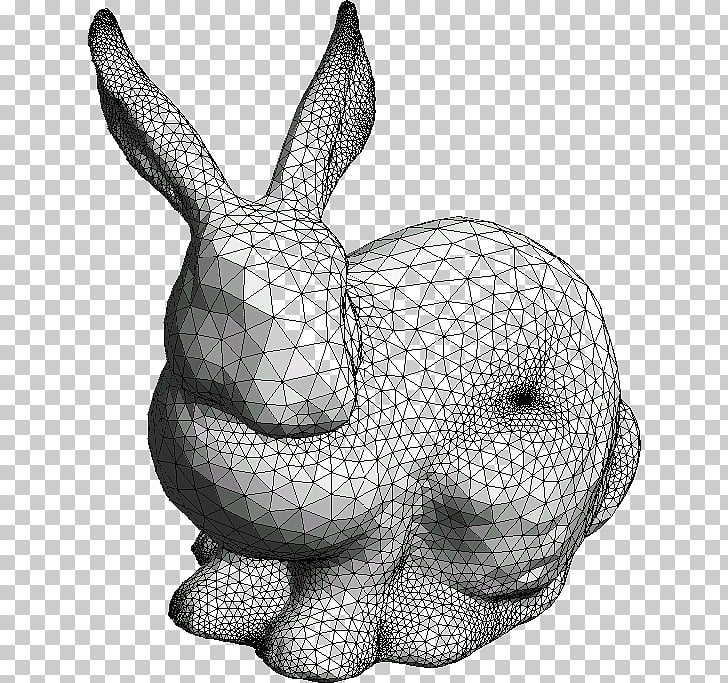
\includegraphics[scale=0.3]{img/rabbit.jpg}
		\caption{Пример треугольной полигональной сетки}
		\label{ris:rabbit}
	\end{figure}
	
	Гранями полигональной сетки обычно являются треугольники, четырёхугольники или другие простые выпуклые многоугольники. У треугольника есть ряд
	особенностей, которые делают его наиболее подходящим для применения в моделировании объектов:
	\begin{enumerate}
		\item[1)] любой треугольник является выпуклым, поэтому разбиение тел на треугольники упрощает рендеринг;
		\item[2)] любой многоугольник может быть разбит на некоторое определённое количество треугольников;
		\item[3)] в треугольнике относительно легко можно восстановить нормаль к исходной
		поверхности, что актуально для алгоритмов закраски;
		\item[4)] невырожденный треугольник всегда
		задает одну плоскость и расположен в одной плоскости.
	\end{enumerate}

	Существуют самые различные способы хранения полигональной сетки трёхмерного объекта. Но так как основная цель данной работы заключается в изучении моделирования реалистичных деревьев, то полигональная сетка будет представлять из себя массив полигонов - треугольников, задающимися координатами вершин.
	
	\subsection{Алгоритмы построения деревьев}
	
	Моделирование объектов природы, в частности лесной растительности, является нетривиальной задачей для большинства известных пакетов 3D-моделирования. В традиционных CAD-системах мы можем получать объекты строгой геометрической формы, которые достаточно хорошо описываются математическими моделями. Объектам живой природы присуща стохастичность в их структуре и огром -ное количество параметров (свет, ветер, гравитация, тип ветвления, осадки), влияющих на их внешний вид. Все это доказывает то, что при моделировании растительности необходимо использовать собственные методы, алгоритмы и подходы.
	
	Все существующие подходы к моделированию деревьев и растений можно условно разделить на три группы:
	
	\begin{itemize}
		\item по определенным математическим правилам и грамматикам;
		\item на основе исходного скелета (эскиза) объекта;
		\item на основе исходного изображения объекта.
	\end{itemize}
	
	Критерием разбиения служит тип входных данных, используемых при моделировании.
	
	При моделировании по определенным математическим правилам и грамматикам входными данными является набор числовых параметров: количество итераций, углы ветвления, радиус ствола, ветвей, коэффициенты уменьшения радиусов и длины ветвей и пр. По данному набору параметров в соответствии c законами ветвления моделируется дерево. Простейшим законом ветвления является модель Хонды.
	
	\subsubsection{Модель Хонды}
	
	Основная идея модели Хонды состоит в следующем:

	\begin{itemize}
		\item сегменты дерева прямые, площадь их поперечного сечения не рассматривается;
		\item в течение итерации материнский сегмент производит два дочерних;

		\item длина двух дочерних сегментов короче материнского в $r1$ и $r2$ раз;

		\item материнский сегмент и два его дочерних находятся в одной плоскости ветвления. Дочерние сегменты выходят из материнского под углами ветвления $\alpha1$ и $\alpha2$
		\item в связи с действием гравитационной силы, плоскость ветвления является «ближайшей к горизонтальной плоскости», иными словами, линия, перпендикулярная материнскому сегменту и лежащая в плоскости ветки — горизонтальная. Исключение делается для веток, присоединенных к главному стволу. В этом случае используется постоянный угол расхождения $\alpha$.
	\end{itemize}

	На рисунке \ref{ris:honda} продемонстрировано ветвление веток из ствола дерева, а также ветвление произвольной ветки.

	\begin{figure}[ht!]
		\centering
		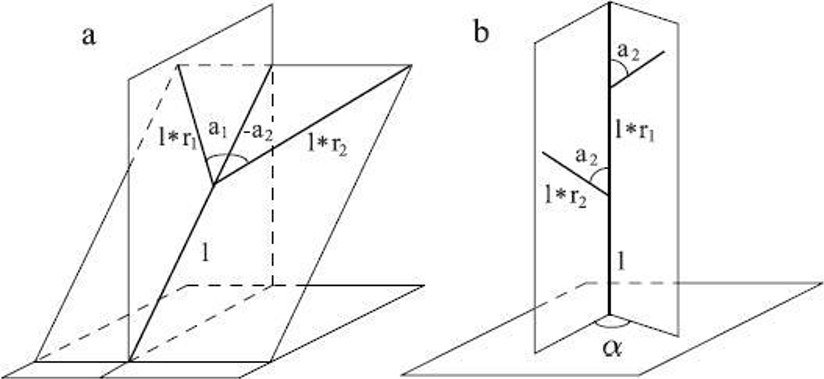
\includegraphics[scale=1]{img/honda.png}
		\caption{Ветвление дерева согласно модели Хонды}
		\label{ris:honda}
	\end{figure}

	\subsubsection{Модель Эоно и Кьюниай}
	
	Модель Эоно и Кьюниай является продолжением модели Хонды. Они предложили несколько улучшений, самым важным из которых был поворот сегментов в определенных направлениях, соответствующих стремлению веток к солнцу, учёту ветра и гравитации. Эоно и Кьюниай использовали прямые линии постоянной или переменной ширины для построения «древесного скелета».
	
	\subsubsection{Стохастические модели}
	
	Эти модели построены по-другому, они разделяют общую парадигму описания структуры деревьев, в частности, расчёт возможностей формирования веток.
	
	
	\subsubsection{Применение L-systems}
	
	В 1968г. Венгерский биолог и ботаник Аристид Линденмайер предложил математическую модель для изучения развития простых многоклеточных организмов, которая позже была расширена и используется для моделирования сложных ветвящихся структур — разнообразных деревьев и цветов. Эта модель получила название L-System. Основная идея L — постоянная перезапись (rewriting) элементов строки. Другими словами, получение сложных объектов путем замены частей простого начального объекта по некоторым правилам. Классическим примером является снежинка. На рисунке \ref{ris:snowflake} initiator — это начальный объект, грани которого заменяются на generator. Далее с новым объектом проделывается то же самое.
	
	\begin{figure}[ht!]
		\centering
		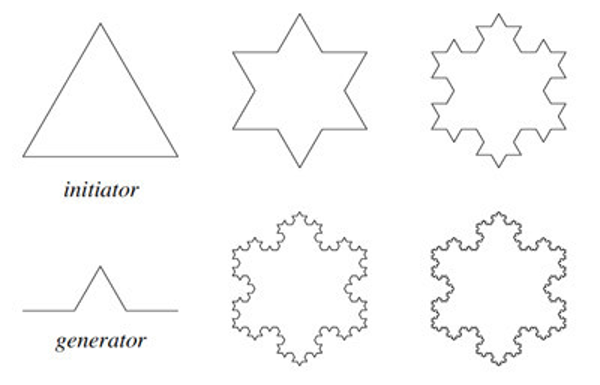
\includegraphics[scale=1]{img/snowflake.png}
		\caption{Классический пример L - снежинка}
		\label{ris:snowflake}
	\end{figure}
	
	Проводя аналогию с фракталами, можно сказать, что L оперирует со строкой символов по специальным правилам, начиная с первоначальной простой аксиомы.

	
	По сути L является грамматикой, но фундаментальное отличие L от формальных грамматик состоит в том, что правила применяются одновременно ко всей строке, к каждому символу, плюс, нет понятий терминальных и нетерминальных символов. То есть «вывод» по этой грамматике может продолжаться бесконечно. Одновременность применения правил очень быстро становится понятна, если учесть откуда пришла эта модель. В биологии каждая клетка растет, делится и развивается параллельно во времени.

	
	Применение L-systems для генерирования деревьев было впервые рассмотрено Эоно и Кьюниай. Для начала, основываясь на формальном определении L, они доказали её непригодность для моделирования высших растений. Но доказательство не относилось к параметрическим L-systems с черепашьей интерпретацией строк. К примеру, L-systems на рисунке 1 выполняет те модели Хонды, в которых один из углов ветвления равен нулю, податливая моноподиальная структура и ясно выраженные главная и боковые оси.

	
	Таким образом, технология L-systems могут играть важную роль как инструмент для биологически-корректного моделирования деревьев и синтеза фотореалистичных изображений.
	
	
	
	\subsubsection{Обоснование выбора алгоритма генерирования каркаса дерева}
	
	Поскольку главной целью данной курсовой работы является анализ моделирования различных 3Д-изображений, то для реализации поставленной задачи используется метод Хонды. В дальнейшем, программу можно будет усовершенствовать, добавляя в нее другие, более реалистичные методы генерации деревьев.
	
	\subsection{Генерация жизненного цикла дерева на основе полученного каркаса}
	
	\subsubsection{Задание индивидуальных характеристик дерева} \label{uninque_ch}
	
	Для того, чтобы иметь возможность генерировать различные виды деревьев, алгоритм генерации деревьев методом Хонда обладает следующими индивидуальными характеристиками дерева:
	\begin{itemize}
		\item точка, из которой будет расти дерево;
		\item угол между двумя главными ветками дерева;
		\item угол между веткой и исходящей из нее веткой;
		\item отношение длины ветки к длине исходящей из нее ветки;
		\item точка на ветке, из которой будет расти следующая ветка;
		\item длина ствола дерева;
		\item радиус ствола;
		\item радиус веток;
		\item цвет дерева.
	\end{itemize}

	Пояснения к характеристикам:
	
	Главными ветками называются ветки, растущие из ствола дерева.
	
	Точка на ветке, из которой будет расти следующая ветка, рассчитывается в алгоритме, используя параметр $start$, определяемый пользователем. Он равен отношению длины ветки к длине части этой ветки. Часть ветки определяет точку, из которой будет расти новая ветка.
	
	Радиус каждого последующего конуса будет вычисляться так, чтобы самая широкая часть этого конуса (ветка дерева) не выходила за границы того конуса, из которого она исходит.
	
	
	\subsubsection{Генерация массива каркасов дерева для каждого момента времени}
	
	Для моделирования процесса роста дерева было решено уменьшать пропорционально индивидуальные характеристики дерева, а именно: радиус ствола, длину ствола, угол между главными ветками, углы между веткой и исходящей из нее веткой, до тех пор пока они не станут меньше заранее заданного минимального значения. 
	
	Таким образом будет сгенерировано определенное количество деревьев с пропорционально уменьшающимися параметрами.
	
	
	\subsection{Построение 3Д-модели на основе получившегося каркаса дерева}
	
	Для визуализации получившегося каркаса дерева каждая ветка и ствол дерева будут представляться в виде конусов, задающихся следующими параметрами: радиусом основания, центром основания, а также вершиной конуса.
	
	Он же в свою очередь будет разбит на определенное количество полигонов (треугольников) \ref{model}, задаваемое пользователем.
	
	
	\subsection{Удаление невидимых поверхностей}
	Одной из наиболее сложных задач в машинной графике является удаление невидимых линий и поверхностей. Все алгоритмы, решающие данную задачу, включают в себя процесс сортировки. Это либо сортировка по расстоянию от точки наблюдения до тела, либо сортировка, основанная на загораживании тел друг другом. Эффективность алгоритмов в большой степени зависит от эффективности алгоритма сортировки.\\
	
	Существует связь между скоростью работы алгоритма и детальностью его результата – ни один алгоритм не может достигнуть хороших показателей в том или другом одновременно.\\
	
	Алгоритмы делятся на 2 типа:
	\begin{enumerate}
	\item[1)]работающие в объектном пространстве;
	\item[2)]работающие в пространстве изображений.
	\end{enumerate}

	Алгоритмы, работающие в объектном пространстве использующте мировую системму координат, обладают высокой точностью. А у алгоритмов, работающих в пространстве изображений система координат связана с дисплеем, и поэтому точность ограничена разрешающей способностью дисплея. Сложность таких алгоритмов составляет $\sim$O($N^2$) и $\sim$O(N$\star$M)  соответственно, при количество объектов - N и количестве пикселей дисплея - M. Но несмотря на то, что $N^2$ < N$\star$M, алгоритмы, работающие в пространстве изображений могут быть эффективнее в силу того, что при растровой реализации близко расположенные пиксели часто обладают одинаковыми свойствами \cite{rod}. Рассмотрим наиболее известные алгоритмы удаления невидимых поверхностей.
	\subsubsection{Алгоритм Робертса}
	Алгоритм Робертса позволяет произвести удаление невидимых линий при помощи математических вычислений. Алгоритм работает в объектном пространстве и состоит из следующих этапов: 
	\begin{enumerate}
		\item[1)]подготовка исходных данных;
		\item[2)]удаление невидимых линий, экранируемых самим телом (для одного тела на этом работа заканчивается);
		\item[3)]удаление линий, экранируемых другими телами;
		\item[4)]удаление линий пересечения тел, экранируемых самими телами, связанными отношением протыкания, и другими телами.
	\end{enumerate}

	Недостатки алгоритма:
	\begin{enumerate}
		\item[1)]для работы алгоритма Робертса необходимо, чтобы все объекты сцены были выпуклыми, если имеются невыпуклые тела, необходимо сначала разбить их на выпуклые;
		\item[2)]вычислительная трудоемкость алгоритма Робертса растет теоретически, как квадрат числа объектов; 
		\item[3)]невозможна реализация теней без использования посторонних методов.
	\end{enumerate}

	Достоинством алгоритма является  точность и быстрота работы математических методов \cite{kur}.
	\subsubsection{Алгоритм Варнока}
	В пространстве изображения рассматривается окно и решается вопрос о том, пусто ли оно, или его содержимое достаточно просто для визуализации. Если содержимое слишком сложно, то окно разбивается на фрагменты до тех пор, пока содержимое фрагмента не станет достаточно простым для визуализации или его размер не достигнет требуемого предела разрешения. В последнем случае информация, содержащаяся в окне, усредняется, и результат изображается с одинаковой интенсивностью или цветом. Пример работы алгоритма Варнока представлен на рис. \ref{ris:varnok}.\\
	\begin{figure}[ht!]
		\centering
		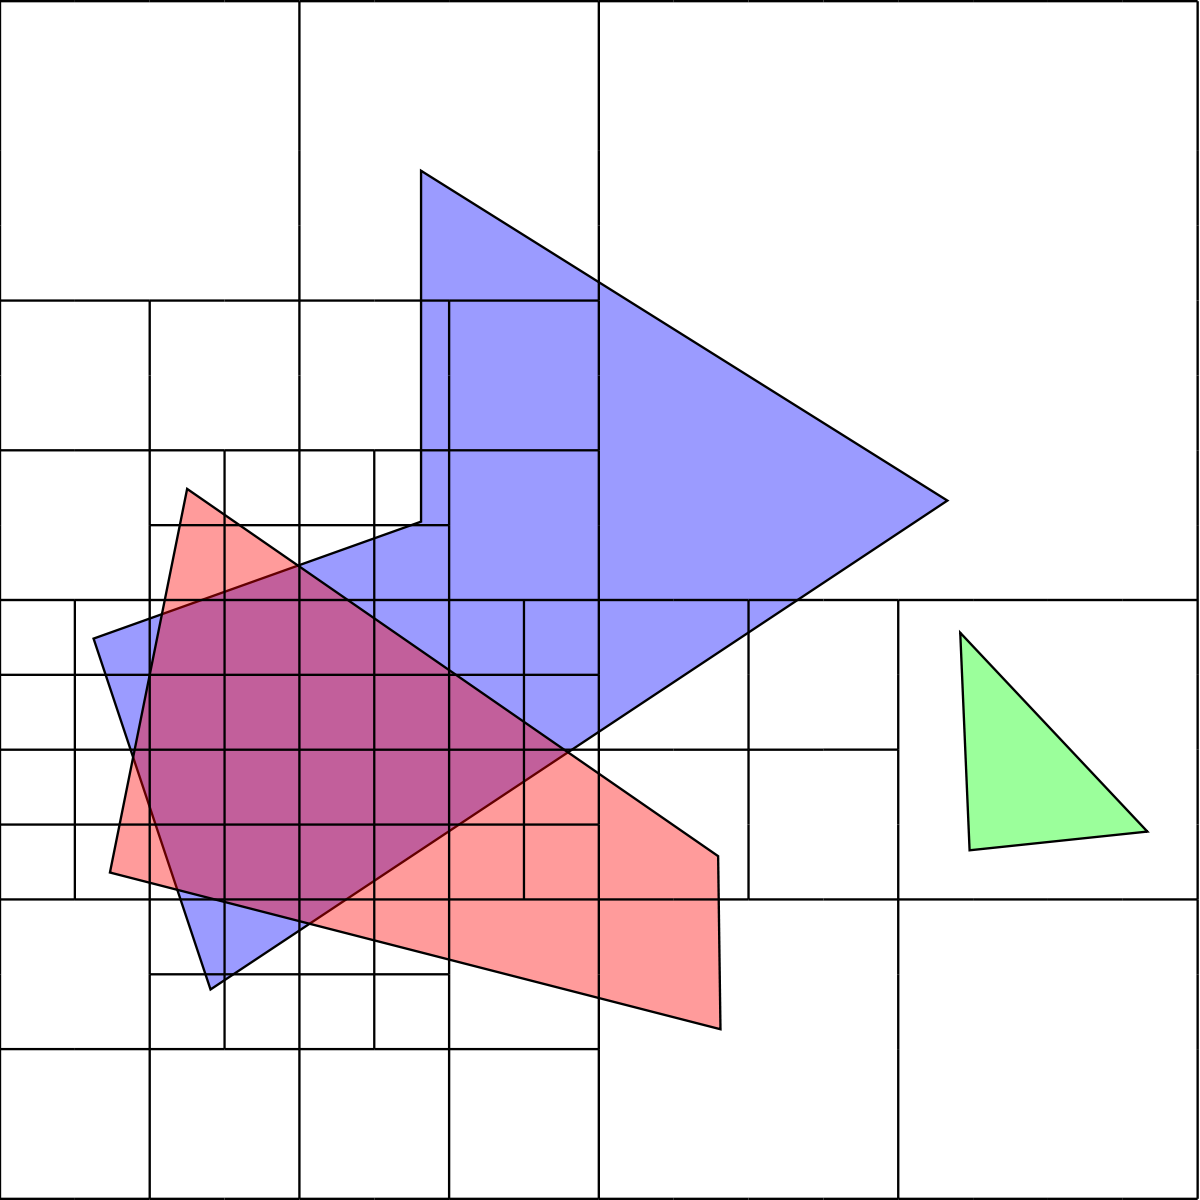
\includegraphics[scale=0.2]{img/varnok.png}
		\caption{Пример работы алгоритма Варнока}
		\label{ris:varnok}
	\end{figure}

	Недостаток алгоритма Варнока заключается в том, что в случае, когда невозможно сразу определить параметры закраски области, разбиение области может проводиться многократно, до тех пор, пока размер области не достигнет одного пиксела. При этом для каждой из полученных подобластей применяется процедура принятия решения.\\
	
	Алгоритм достаточно прост с точки зрения понимания, однако может потребоваться большое количество разбиений, соответственно потребуется много времени на анализ и отображение содержимого всего окна. В случае отрисовки сложных сцен со множеством объектов алгоритм становится неэффективным.
	\subsubsection{Алгоритм, использующий Z-буфер}
	Данный алгоритм является одним из простейших алгоритмов удаления невидимых линий и поверхностей. Алгоритм работает в пространстве изображений.\\
	
	Идея Z-буфера является простым обобщением идеи о буфере кадра. Буфер кадра используется для запоминания атрибутов (интенсивности) каждого пиксела в пространстве изображения. Z-буфер - это отдельный буфер глубины, используемый для запоминания координаты Z или глубины каждого видимого пиксела в пространстве изображения. В процессе работы глубина или значение Z каждого нового пиксела, который нужно занести в буфер кадра, сравнивается с глубиной того пиксела, который уже занесен в Z-буфер. Если это сравнение показывает, что новый пиксел расположен впереди пиксела, находящегося в буфере кадра, то новый пиксел заносится в этот буфер и, кроме того, производится корректировка Z-буфера новым значением Z. Если же сравнение дает противоположный результат, то никаких действий не производится. Вычислительная сложность данного алгоритма, которая равна O(N*M*K), где M*N – количество пикселей в буфере кадра, K – количество многоугольников. На рис.\ref{ris:zbuffer} представлен пример работы алгорима, использующего z-буфер.\\
	\begin{figure}[ht!]
		\centering
		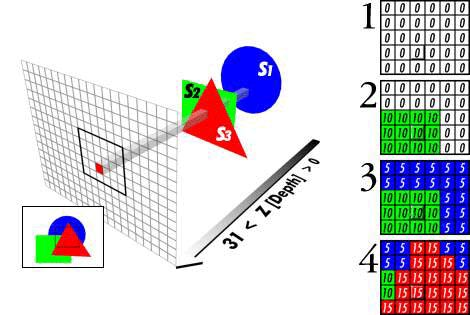
\includegraphics[scale=0.7]{img/zbuffer.jpg}
		\caption{Пример работы алгоритма, использующего z-буфер}
		\label{ris:zbuffer}
	\end{figure}
	
	Главное преимущество алгоритма – его простота. Также, этот алгоритм делает тривиальной визуализацию пересечений поверхностей. Кроме того, объекты сцены могут рассматриваться в произвольном порядке, что позволяет не тратить время на сортировку объектов по глубине.\\
	
	Недостатком алгоритма является большой объем требуемой памяти для хранения буферов, трудоемкость и высокая стоимость устранения лестничного эффекта и трудоемкость реализации эффектов прозрачности и просвечивания.\\
	\subsubsection{Обоснование выбора алгоритма удаления невидимых линий и поверхностей}
	В проекте используется алгоритм, использующий Z-буфер, так как данный алгоритм позволяет строить сцены любой сложности, а также достаточно быстро работает за счет отсутствия сложных вычислений. Так как на сегодняшний день размер оперативной памяти достаточно велик, использование большого объема памяти не является существенным недостатком применения данного алгоритма в программном продукте.
	\subsection{Алгоритмы закраски}
	Изображение формируется в результате отражения падающего на поверхность объектов света, интенсивность и цвет которого необходимо рассчитать. Для
	вычисления этих параметров используют методы закраски поверхностей.

	\subsubsection{Алгоритм плоской закраски}
	Алгоритм плоской закраски довольно прост. Сперва вычисляется нормаль к текущему многоугольнику, зачем на основе значения нормали в соответствии с выбранной моделью освещения считается интенсивность цвета всего многоугольника. Такой метод закрашивания обладает высокой скоростью работы, но на визуализированной модели заметны переходы между гранями.\\
	Недостаток данного алгоритма заключается в том, что его применение ограничено тремя условиями:
	\begin{enumerate}
		\item[1)]источник света находится в бесконечности;
		\item[2)]наблюдатель находится в бесконечности; 
		\item[3)]закрашиваемый многоугольник является реально существующим многоугольником, а не результатом аппроксимации поверхностей.
	\end{enumerate}
	\subsubsection{Алгоритм закраски Гуро}
	Метод Гуро основан на идее закрашивания грани не сплошным цветом, а
	плавно изменяющимися оттенками. При данном виде закраски интерполируется значение интенсивности, что позволяет получить сглаженное изображение \cite{kur}.\\
	
	Процесс закраски Гуро можно разделить на 4 этапа:
	\begin{enumerate}
		\item[1)]вычисление векторов нормалей к каждой грани;
		\item[2)]вычисление векторов нормалей к каждой вершине грани путем усреднения
		нормалей к граням;
		\item[3)]вычисление значений интенсивности в вершинах грани;
		\item[4)] закраска многоугольника путем интерполяции значений интенсивности в вершинах сначала вдоль каждого ребра, а затем и между ребрами вдоль каждой сканирующей строки.
	\end{enumerate}

	Закраска методом Гуро обеспечивает непрерывность значений интенсивноти
	вдоль границ многоугольников, но не обеспечивает непрерывности изменения интенсивности, поэтому при использовании данного алгоритма возможно появление полос Маха. Также на некоторых участках поверхность будет выглядеть плоской, поскольку при линейной интерполяции значение интенсивности на этих участках может получится равной.
	\subsubsection{Алгоритм закраски Фонга}
	Метод Фонга базируется на той же идее, что и метод Гуро, но при закраске
	здесь интерполируется не значения интенсивности, а вектор нормали. Затем он используется в моделе освещения для вычисления интенсивности. Это позволяет уменьшить количество полос Маха и добиться лучшей локальной аппроксимации кривизны поверхности. Также метода Фонга, работая с нематовыми поверхностями, выдаёт более реалистичное изображение по сравнению с методом Гуро за счёт наличия зеркальных бликов \cite{kur}.\\
	
	Процесс закраски Фонга можно разделить на 5 этапов:
	\begin{enumerate}
		\item[1)]вычисление векторов нормалей к каждому полигону;
		\item[2)]вычисление векторов нормалей к каждой вершине;
		\item[3)]вычисление значений нормалей вдоль ребер путем интерполяции значений
		интенсивности в вершинах;
		\item[4)]вычисление нормали вдоль сканирующей строки;
		\item[5)]закраска многоугольника путем использования полученной нормали.
	\end{enumerate}

	Закраска методом Фонга позволяет частично устранить недостатки закраски
	методом Гуро и получить более реалистичное изображение, однако она сложнее в
	реализации и требует больших вычислительных затрат.
	
	\subsubsection{Обоснование выбора алгоритма закраски}
	В курсовом проекте используется алгоритм тонировки Гуро, так как он требует меньшего количества вычислений, чем алгоритм закраски Фонга и не сильно уступает в получении реалистичностого изображения по сравнению с плоским алгоритмом закраски.
	
	\subsection{Требования к программному обеспечению}
	Программное обеспечение должно реализовывать возможность генерации, а также моделирования дерева, задающееся следующими индивидуальными характеристиками (подробнее в: \ref{uninque_ch}):
	\begin{itemize}
		\item точка, из которой будет расти дерево;
		\item угол между двумя главными ветками дерева;
		\item угол между веткой и исходящей из нее веткой;
		\item отношение длины ветки к длине исходящей из нее ветки;
		\item точка на ветке, из которой будет расти следующая ветка;
		\item длина ствола дерева;
		\item радиус ствола;
		\item радиус веток;
		\item цвет дерева.
	\end{itemize}
	
	Моделирование дерева должно использовать такие алгоритмы как закраска Гуро и z-буфер.
	
	Пользователь должен иметь возможность загружать, сохранять индивидуальные характеристики дерева, перемещать, вращать и масштабировать как сам 3Д-объект, так и камеру. Также должна быть возможность добавления новых камер (точек обзора). Пользователь должен иметь возможность свободно переключаться между этими камерами, чтобы удобно рассматривать дерево с разных ракурсов.
	
	Помимо этого, пользователь должен иметь возможность менять вектор направления света, а также его интенсивность.
	
	\subsection{Выводы по аналитическому разделу}
	В данном разделе был произведён анализ предметной области, методов и
	алгоритмов, которые необходимы для решения поставленной задачи.\\

	В качестве модели объектов была выбрана полигональная сетка, хранящаяся в массиве полигонов - треугольников, задающимися координатами вершин.
	
	В качестве алгоритма удаления невидимых граней был выбран алгоритм,
	использующий z-буфер, который работает достаточно быстро за счет отсутствия сложных вычислений. Алгоритм z-буфера имеет недостаток, заключающийся в использовании большого объема памяти. Однако его можно считать несущественным, поскольку размер оперативной памяти на сегодняшний день считается достаточно большим.
	
	В качестве алгоритма закраски был выбран алгоритм тонировки Гуро, так как он требует меньшего количества вычислений, чем алгоритм закраски Фонга и не сильно уступает в получении реалистичностого изображения по сравнению с плоским алгоритмом закраски.
	
	В качестве алгоритма генерации реалистичного каркаса дерева был выбран алгоритм, основывающийся на модели Хонды. 
	
	Каждая ветка дерева будет представлять из себя конус, разбитый на определенное количество полигонов.
	
	
	\newpage
	\section{Конструкторский раздел}
	В данном разделе будут более подробно описаны выбранные в аналитическом разделе алгоритмы, будут перечислены основные типы и структуры данных, использующиеся в проекте, и представлена диаграмма классов архитектуры проекта.
	\subsection{Процесс отрисовки изображения}
	\subsubsection{Z-буфер}
	В процессе работы алгоритма z-буфера анализируется глубина каждого пикселя в пространстве изображения. Если пиксели двух рисуемых объектов перекрываются, то их значения глубины сравниваются. Если это сравнение показывает, что
	новый пиксел расположен ближе к наблюдателю, чем пиксел, уже находящийся в
	буфере кадра, то новое значение координаты z заносится в z-буфер, корректируя
	значение интенсивности, находящееся в буфере кадра. Если же сравнение дает противоположный результат, то никаких действий не производится. По сути, алгоритм
	является поиском по х и у наибольшего значения функции z(х,у).\\
	Формальное описание алгоритма z-буфера:
	\begin{enumerate}
		\item[1)]заполнить буфер кадра фоновым значением интенсивности или цвета;
		\item[2)]заполнить z-буфер минимальным значением z;
		\item[3)]преобразовать каждый многоугольник в растровую форму в произвольном
		порядке;
		\item[4)]для каждого пикселя в многоугольнике вычислить его глубину z(x,y);
		\item[5)]сравнить глубину z(х,у) со значением z-буфера, хранящимся в z-буфере в
		этой же позиции;
		\item[6)]если z(х,у) > z-буфер(х,у), то записать атрибут этого многоугольника (интенсивность, цвет и т. п.) в буфер кадра и заменить z-буфер(х,у) на z(х,у). В противном
		случае никаких действий не производить.
	\end{enumerate}
	На рис. \ref{ris:z}  представлен полный процесс отрисовки изображения.
	\begin{figure}[ht!]
		\centering
		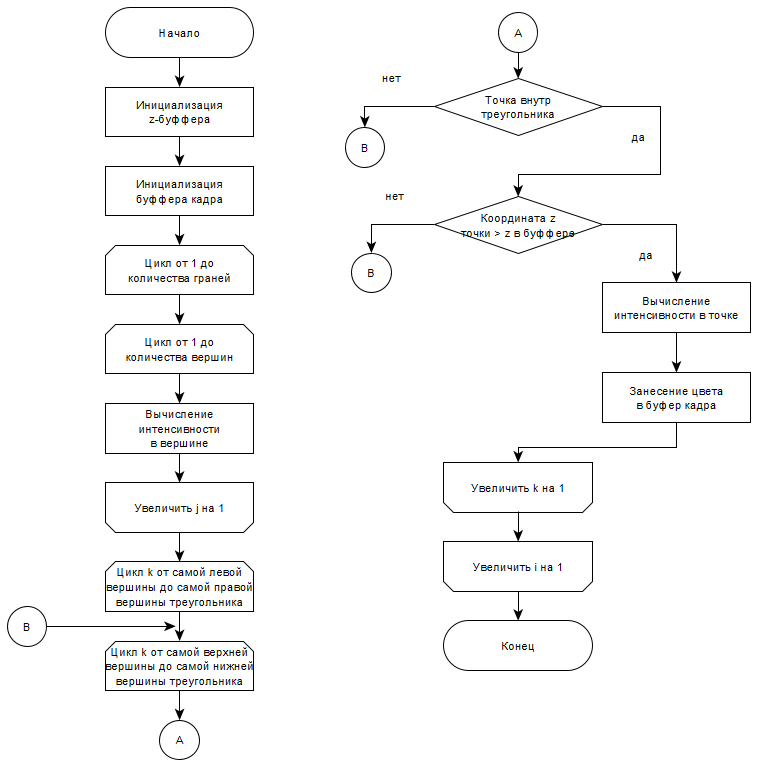
\includegraphics[scale=1]{img/z.PNG}
		\caption{Процесс отрисовки изображения}
		\label{ris:z}
	\end{figure}
	
	\newpage
	
	\subsubsection{Закраска Гуро}
	
	Метод закраски, который основан на интерполяции интенсивности и известен как метод Гуро (по имени его разработчика), позволяет устранить дискретность изменения интенсивности. Процесс закраски по методу Гуро осуществляется в четыре этапа:
	
	\begin{enumerate}
		\item Вычисляются нормали ко всем полигонам;
		\item Определяются нормали в вершинах путем усреднения нормалей по всем полигональным граням, которым принадлежит вершина;
		\item Используя нормали в вершинах и применяя произвольный метод закраски, вычисляются значения интенсивности в вершинах;
		\item Каждый многоугольник закрашивается путем линейной интерполяции значений интенсивностей в вершинах сначала вдоль каждого ребра, а затем и между ребрами вдоль каждой сканирующей строки.
	\end{enumerate}

	Линейная интерполяция осуществляется следующим образом:
	Интенсивность вдоль отрезка AB в некоторой точке C вычисляется по формуле \cite{Guro}:
	
	Схема алгоритма закраски Гуро приведена на рисунке \ref{ris:Guro}.
	
	\begin{figure}[ht!]
		\centering
		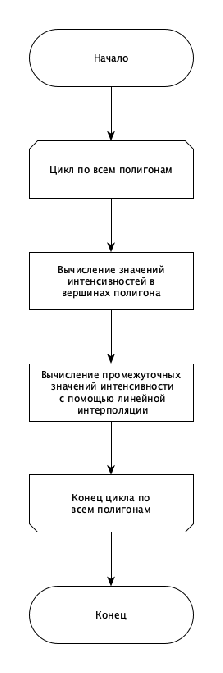
\includegraphics[scale=1.5]{img/Guro.eps}
		\caption{Схема алгоритма закраски методом Гуро}
		\label{ris:Guro}
	\end{figure}
	
	
	\subsection{Генерация каркаса дерева}
	На рисунке \ref{ris:alg_Honda} представлена схема алгоритма генерации дерева, использующего модель Хонды.
	
	\newpage
	
	\begin{figure}[ht!]
		\centering
		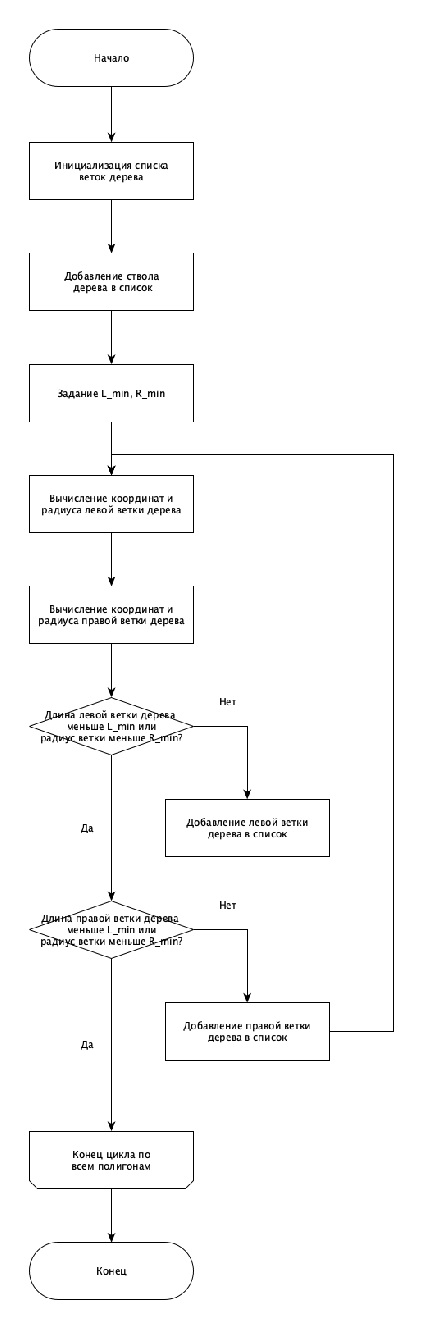
\includegraphics[scale=1.1]{img/Honda.eps}
		\caption{Схема алгоритма генерации дерева, использующего модель Хонды}
		\label{ris:alg_Honda}
	\end{figure}
	
	\subsection{Построение 3Д-модели на основе получившегося каркаса дерева}
	
	Для представления получившегося каркаса дерева в виде совокупности конусов, разбитых на определенное количество полигонов, необходимо:
	\begin{itemize}
		\item переместить $i$-ую ветку в начало координат;
		\item повернуть ее так, чтобы она совпала с осью OZ \cite{algo_rotate};
		\item Разбить конус на определенное количество треугольников.
	\end{itemize}
	
	\subsection{Трехмерные аффинные преобразования}
	В процессе работы программы возникает необходимость преобразования объектов сцены – их поворота. Для трехмерного пространства любое аффинное преобразование может быть представлено последовательностью простейших операций.
	 
	Ниже приведены уравнения поворота относительно осей x (\ref{x}), y (\ref{y}) и z (\ref{z}) на угол $\phi$.
	\begin{equation}
	\begin{cases}
	X = x\\
	Y = y\cdot\cos\phi + z\cdot\sin\phi\\
	Z = -y\cdot\sin\phi + z\cdot\cos\phi\\
	\end{cases}
	\label{x}
	\end{equation}
	
	\begin{equation}
	\begin{cases}
	X = x\cdot\cos\phi + z\cdot\sin\phi\\
	Y = y\\
	Z = -x\cdot\sin\phi + z\cdot\cos\phi\\
	\end{cases}
	\label{y}
	\end{equation}
	
	\begin{equation}
	\begin{cases}
	X = x\cdot\cos\phi + y\cdot\sin\phi\\
	Y = -x\cdot\sin\phi + y\cdot\cos\phi\\
	Z = z\\
	\end{cases}
	\label{z}
	\end{equation}
	
	Поворот объекта относительно одной из координатных осей также можно представить в виде матриц.
	Ниже представлены три матрицы поворота объекта относительно оси x, y и z соответственно.
	$$\begin{pmatrix}
		1 & 0 & 0 & 0\\
		0 & \cos\phi & \sin\phi & 0\\
		0 & -\sin\phi & \cos\phi & 0\\
		0 & 0 & 0 & 1\\
		\label{mtx_x}
	\end{pmatrix} $$
	
	$$\begin{pmatrix}
	\cos\phi & 0 & \sin\phi & 0\\
	0 & 1 & 0 & 0\\
	-\sin\phi & 0 & \cos\phi & 0\\
	0 & 0 & 0 & 1\\
	\label{mtx_y}
	\end{pmatrix} $$
	
	$$\begin{pmatrix}
	\cos\phi & \sin\phi & 0 & 0\\
	-\sin\phi & \cos\phi & 0 & 0\\
	0 & 0 & 1 & 0\\
	0 & 0 & 0 & 1\\
	\label{mtx_z}
	\end{pmatrix} $$
	
	\subsection{Используемые типы и структуры данных}
	В реализованной программе используются некоторые базовые типы C++, такие как integer и double. Также применяется тип данных QVector для хранения объектов сцены, буфера кадра и реализации алгоритма, использующего z-буфера.
	
	Кроме того, в программе используются структуры данных, описывающие
	матрицу и математический вектор, который предусматривает операции векторного
	и скалярного умножения, нахождения длины вектора, нормализации;  а также бинарное дерево - для реализации алгоритма генерации деревьев.
	\newpage
	\subsection{Общая архитектура проекта}
	Архитектура проекта сформирована в соответствии с канонами объектноориентированного программирования. На рис. \ref{ris:model} представлена диаграмма классов архитектуры проекта.
	\begin{figure}[ht!]
		\centering
		\includegraphics[scale=1]{img/diagram.eps}
		\caption{Диаграмма классов программы}
		\label{ris:model}
	\end{figure}

	\begin{itemize}
		\item Widget – основной класс, работающий с окном приложения;
		\item Growth\_factory - класс генерации жизненного цикла дерева, реализующий шаблон проектирования «Фабрика» \cite{patterns}.
		\item Object\_factory - класс построения 3Д-модели на основе получившегося каркаса дерева, реализующий шаблон проектирования «Фабрика» \cite{patterns}.
		\item Tree\_factory - класс генерации дерева, реализующий шаблон проектирования «Фабрика» \cite{patterns}.
		\item Action - класс, содержащих информацию о команде, которая передается через Facade.
		\item Facade - класс, реализующий шаблон проектирования «Фасад» \cite{patterns}.
		\item Drawer - класс отрисовщика, содержащий методы, которые реализуют отображение буфера кадра на экране.
		\item DrawManager -  класс менеджера отрисовщика; содержит методы отрисовки модели.
		\item ModelManager - класс, применяющий преобразования перемещения, масштабирования и поворота к моделям через ModelTransformator.
		\item CameraManager - класс, применяющий преобразования перемещения, масштабирования и поворота к камерам через CameraTransformator.
		\item Camera - класс камеры, позволяющий изменять параметры перемещения, масштабирования и поворота камеры.
		\item CompositeObject - класс, реализующий шаблон проектирования «Компоновщик» \cite{patterns}.
		\item Edge - класс ветки дерева, содержит номера вершин веток и радиус ветки.
		\item Model - класс каркаса дерева, содержит Edge и Node.
		\item Node - класс точки, содержит вершину точки и цвет.
		\item Transformed\_model - класс, содержащий полигональную модель дерева.
		\item Triangle - класс треугольника, содержит вершины треугольника и цвет вершин.
		\item Scene - класс, позволяющий добавлять, удалять модели, камеры сцены, обеспечивает взаимодействие с CompositeObject.
		\item FileUploader - класс загрузщика модели из файла; содержит методы,
		реализующие работу с файлом; выполняет загрузку считанных параметров в класс Tree\_factory.
		\item GenerateUploader - класс созданий модели, выполняет загрузку параметров в класс Tree\_factory.
		\item ModelTransformator - класс применяющий преобразования перемещения, масштабирования и поворота к модели.
		\item CameraTransformator - класс применяющий преобразования перемещения, масштабирования и поворота к камере.
		\item Z\_Buffer - содержит методы, реализующие удаление невидимых
		линий и поверхностей алгоритмом z-буфера.
	\end{itemize}

	\subsection{Выводы по конструкторскому разделу}
	В данном разделе были даны формальные описания алгоритмов z-буфера, Гуро, Хонды, полигонализации конусов; выбранных в аналитическом разделе. 
	
	Также были приведены математические формулы поворота объекта относительно каждой из трех координатных осей. Были перечислены основные типы и
	структуры данных, использующиеся в проекте, и представлена диаграмма классов архитектуры проекта.

	\newpage
	\section {Технологический раздел}
	В данном разделе будут рассмотрены средства, использованные в процессе
	разработки для реализации поставленных задач, информация о сборке и запуске проекта, будут представлены основные функции интерфейса, а также приведены
	примеры работы программы при различных параметрах.
	\subsection {Средства реализации}
	Для реализации программы был использован язык программирования C++, стандарт C++17 ~\cite{C}. С++ имеет достаточный функционал в стандартных библиотеках и является высокопроизводительным языком, что очень важно при реализации задач компьютерной графики из-за высокой нагрузки на аппаратное обеспечение.\\
	
	Проект был выполнен в среде QtCreator\cite{Qt}. В качестве графической оболочки была выбрана QtGraphics, которая предоставляет поверхность для управления и взаимодействия с большим количеством пользовательских графических 2D объектов, что важно при отрисовки большого количества многоугольников полигональной сетки. Платформа включает в себя архитектуру распространения событий, которая позволяет использовать возможности взаимодействия элементов на сцене.
	\subsection {Сборка и запуск проекта}
	Для компиляции и сборки проекта используется gcc и системы сборки
	qmake\cite{Qt}, которая автоматически генерирует make-файлы, основываясь на информации в файлах проекта. Также для корректной сборки приложения необходимы основные библиотеки QtGraphics, стандартные библиотеки С++ и доступ к пространству имен std.
	\newpage
	\subsection{Интерфейс программы}
	
	Интерфейс программы состоит из окна вывода изображения, имеющего фиксированный размер 700x700 пикселей, и набора виджетов, позволяющих пользователю взаимодействовать с программой (рисунок \ref{ris:prog}).
	\begin{figure}[h!]
		\centering
		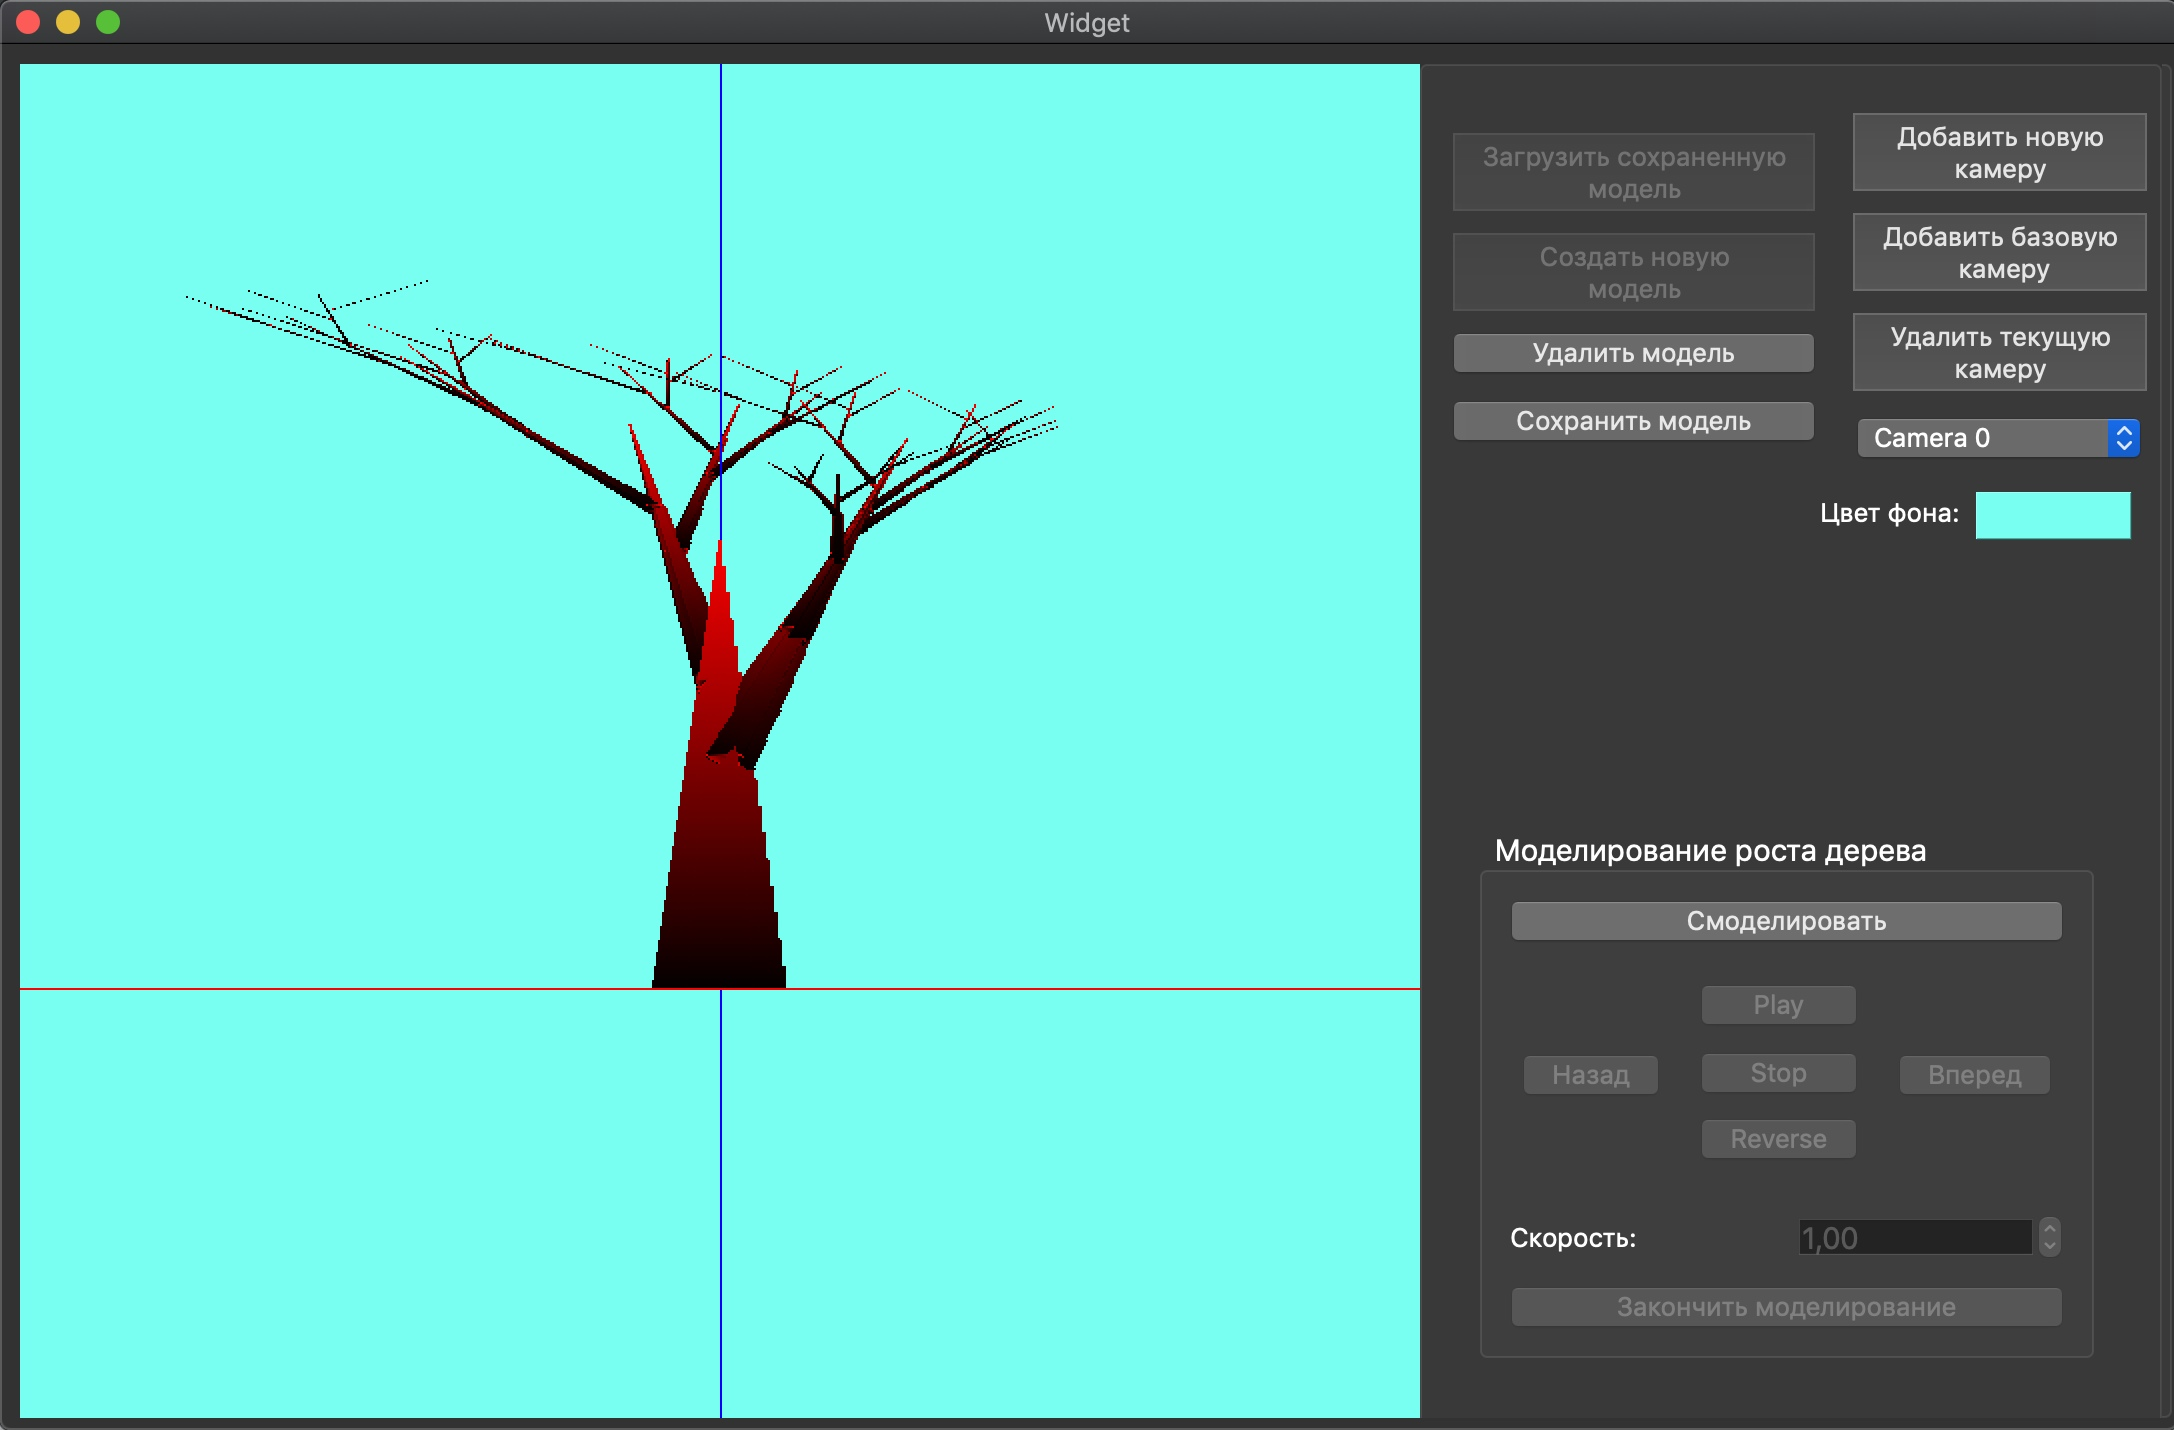
\includegraphics[scale=0.2]{img/tree.JPG}
		\caption{Интерфейс программы}
		\label{ris:prog}
	\end{figure}
	
	\newpage
	При запуске программы пользователю предоставлется возможность выбрать, хочет ли он загрузить готовые параметры дерева, или же он хочет задать их вручную. Если он выбирает загрузку параметров, то перед ним выскакивает каталог файлов, из которых ему необходимо будет выбрать модель.	В другом случае перед ним появится окно с параметрами дерева, которое будет сгенерировано, их необходимо заполнить (рисунок \ref{ris:params}).
	\begin{figure}[h!]
		\centering
		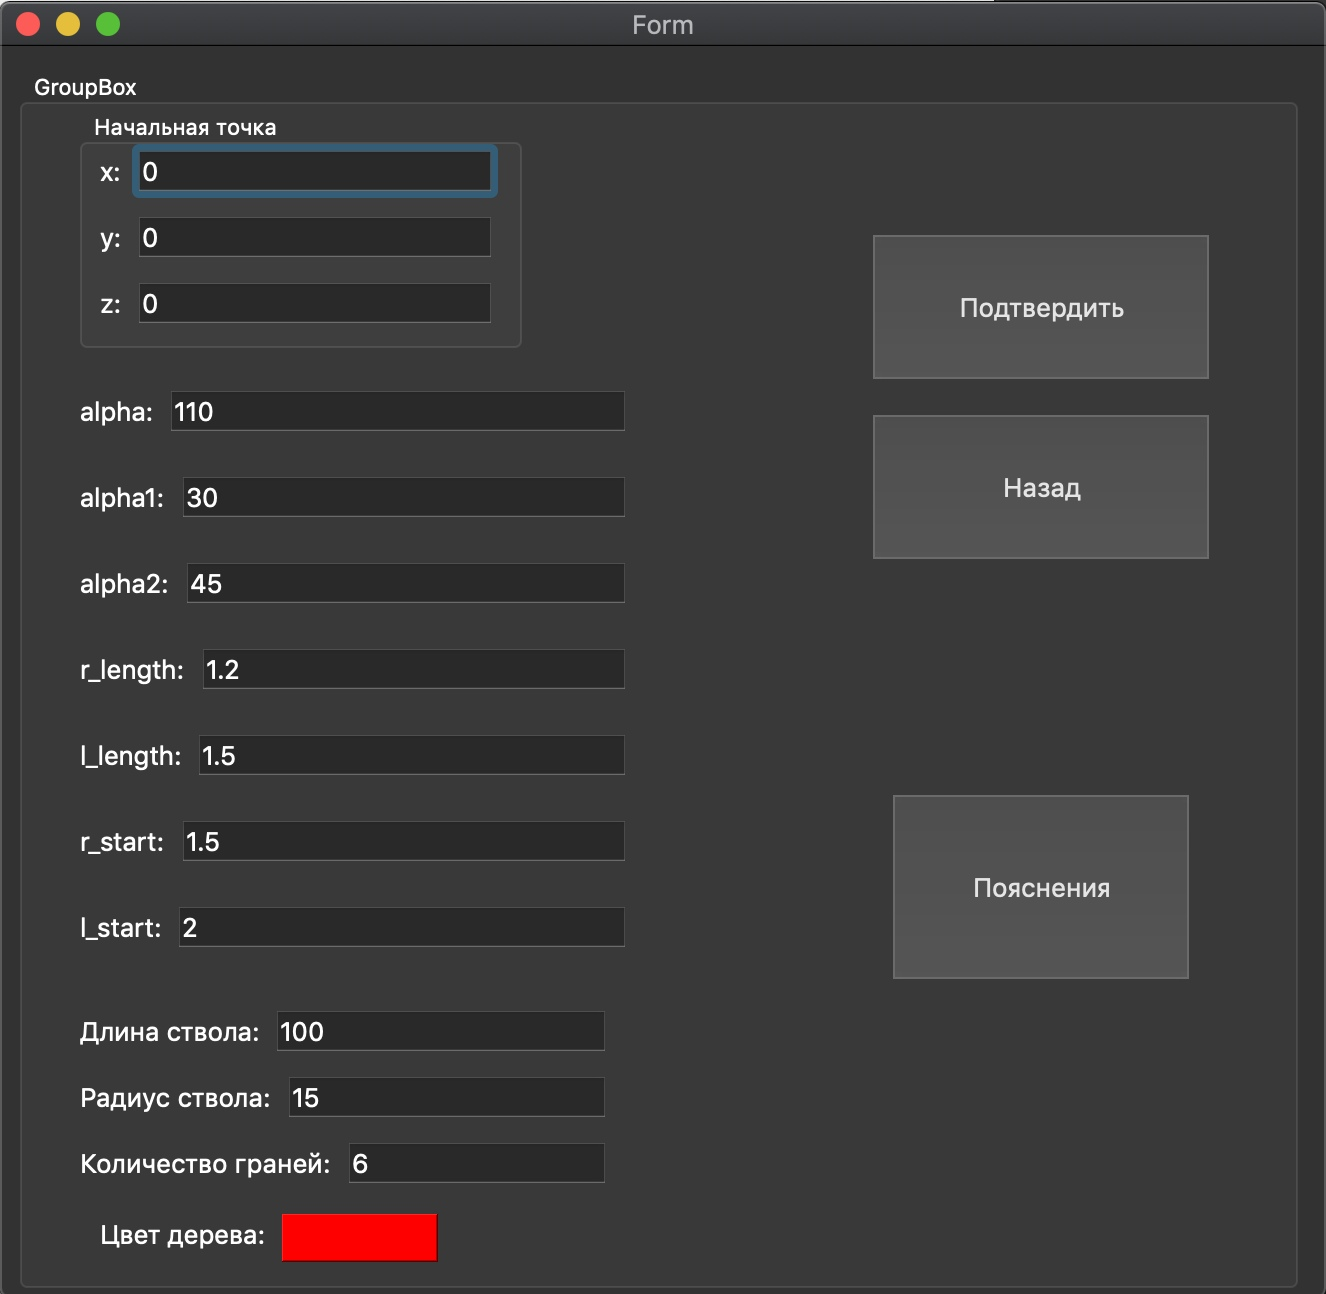
\includegraphics[scale=0.2]{img/params.JPG}
		\caption{Параметры дерева}
		\label{ris:params}
	\end{figure}
	
	После нажатия кнопки "Подтвердить" на экран выводится сгенерированное дерево, которое можно поворачивать, масштабировать и перемещать, используя клавиши на клавиатуре (подробнее в горячих клавишах программы: \ref{print}).
	
	Помимо вращения самой модели, обеспечивается возможность добавление и удаление новых камер, а также переключение между ними с помощью кнопок: 
	\begin{enumerate}
		\item <<Добавить камеру>> - добавляет камеру, зафиксированную в положении, что и предыдущая камера;
		\item <<Удалить камеру>> - удаляет текушую камеру;
		\item <<Добавить базовую камеру>> - добавляет камеру, направленную в начало координат;
		\item <<Camera$i$>> - позволяет переключаться между камерами.
	\end{enumerate}

	Камеры как и сам объект можно вращать, приближать и перемещать используя те же горячие клавиши после однократного нажатия клавищи Command (подробнее о горячих клавишах программы: \ref{print}).
	
	Программа предоставляет возможность пользователю изменять вектор направления падения лучей источника света и интесивность источника света, используя те же горячие клавиши после двухкратного нажатия клавищи Command (подробнее о горячих клавишах программы: \ref{print}).

	В нижней правой части экрана присутствует необходимое меню для моделирования роста дерева. При нажатии на кнопку "Смоделировать" генерируется дерево "в более ранних стадиях его развития", после чего "зерно" дерева выводится на экран.
	
	После нажатия на кнопку "Play" происходит визуализация жизненного цикла дерева путем последовательной смены 3Д-объектов одного за другим. При этом пользователь все также имеет возможность перемещать, поворачивать, масштабировать само дерево или камеру в процессе визуализации. Пользователь может в любой момент нажать на кнопку "Stop", после чего моделирование жизненного цикла дерева будет приостановлено. 
	
	После нажатия на кнопку "Reverse" происходит обратная визуализация жизненного цикла дерева путем последовательной смены 3Д-объектов одного за другим. Пользователь может замедлить или увеличить скорость роста дерева используя счетчик, расположенный рядом с кнопкой "Reverse".
	
	В качестве альтернативы кнопкам "Play" и "Reverse" пользователь может воспользоваться кнопками "Вперед" или "Назад", чтобы более детально рассмотреть каждый этап роста дерева.
	\newpage
	
	\subsection{Горячие клавиши программы} \label{print}
	Ниже приведен список кнопок на клавиатуре, выполняющих ту или иную функцию:
	\begin{enumerate}
		\item A - перемешение вдоль оси OX в отрицательном направлении;
		\item D - перемешение вдоль оси OX в положительном направлении;
		\item S - перемешение вдоль оси OY в положительном направлении;
		\item W - перемешение вдоль оси OY в отрицательном направлении;
		\item Q - перемешение вдоль оси OZ в положительном направлени;
		\item E - перемешение вдоль оси OZ в отрицательном направлени;
		\item R - масштабирование (увеличение);
		\item T - масштабирование (уменьшение);
		\item Z - поворот вокруг оси OX в положительном направлении;
		\item X - поворот вокруг оси OY в положительном направлении;
		\item C - поворот вокруг оси OZ в положительном направлении;
		\item V - поворот вокруг оси OX в отрицательном направлении;
		\item B - поворот вокруг оси OY в отрицательном направлении;
		\item N - поворот вокруг оси OZ в отрицательном направлении;
		\item Command - при первом нажатии этой кнопки все предыдущие кнопки начинают работать с камерой, а не с объектом (до этого перемещался, масштабировался и вращался объект с помощью предыдущих кнопок); при втором нажатии этой кнопки кнопки с Z-N начинают работать с освещением, при третьем нажатии - с объектом и так далее; 
		\item O - увеличить яркость освещения;
		\item L - уменьшить яркость освещения;
	\end{enumerate}
	
	\subsection{Тестирование программы}
	На рисунках \ref{ris:ex1}, \ref{ris:ex2}, \ref{ris:ex3}, \ref{ris:ex4} и \ref{ris:ex5} представлены примеры работы программы для различных параметров генерации дерева. Примеры демонстрируют результаты выполнения программы при различных положениях объектов, камер и источника света. 
	
	\newpage
	
	\begin{figure}[ht!]
		\centering
		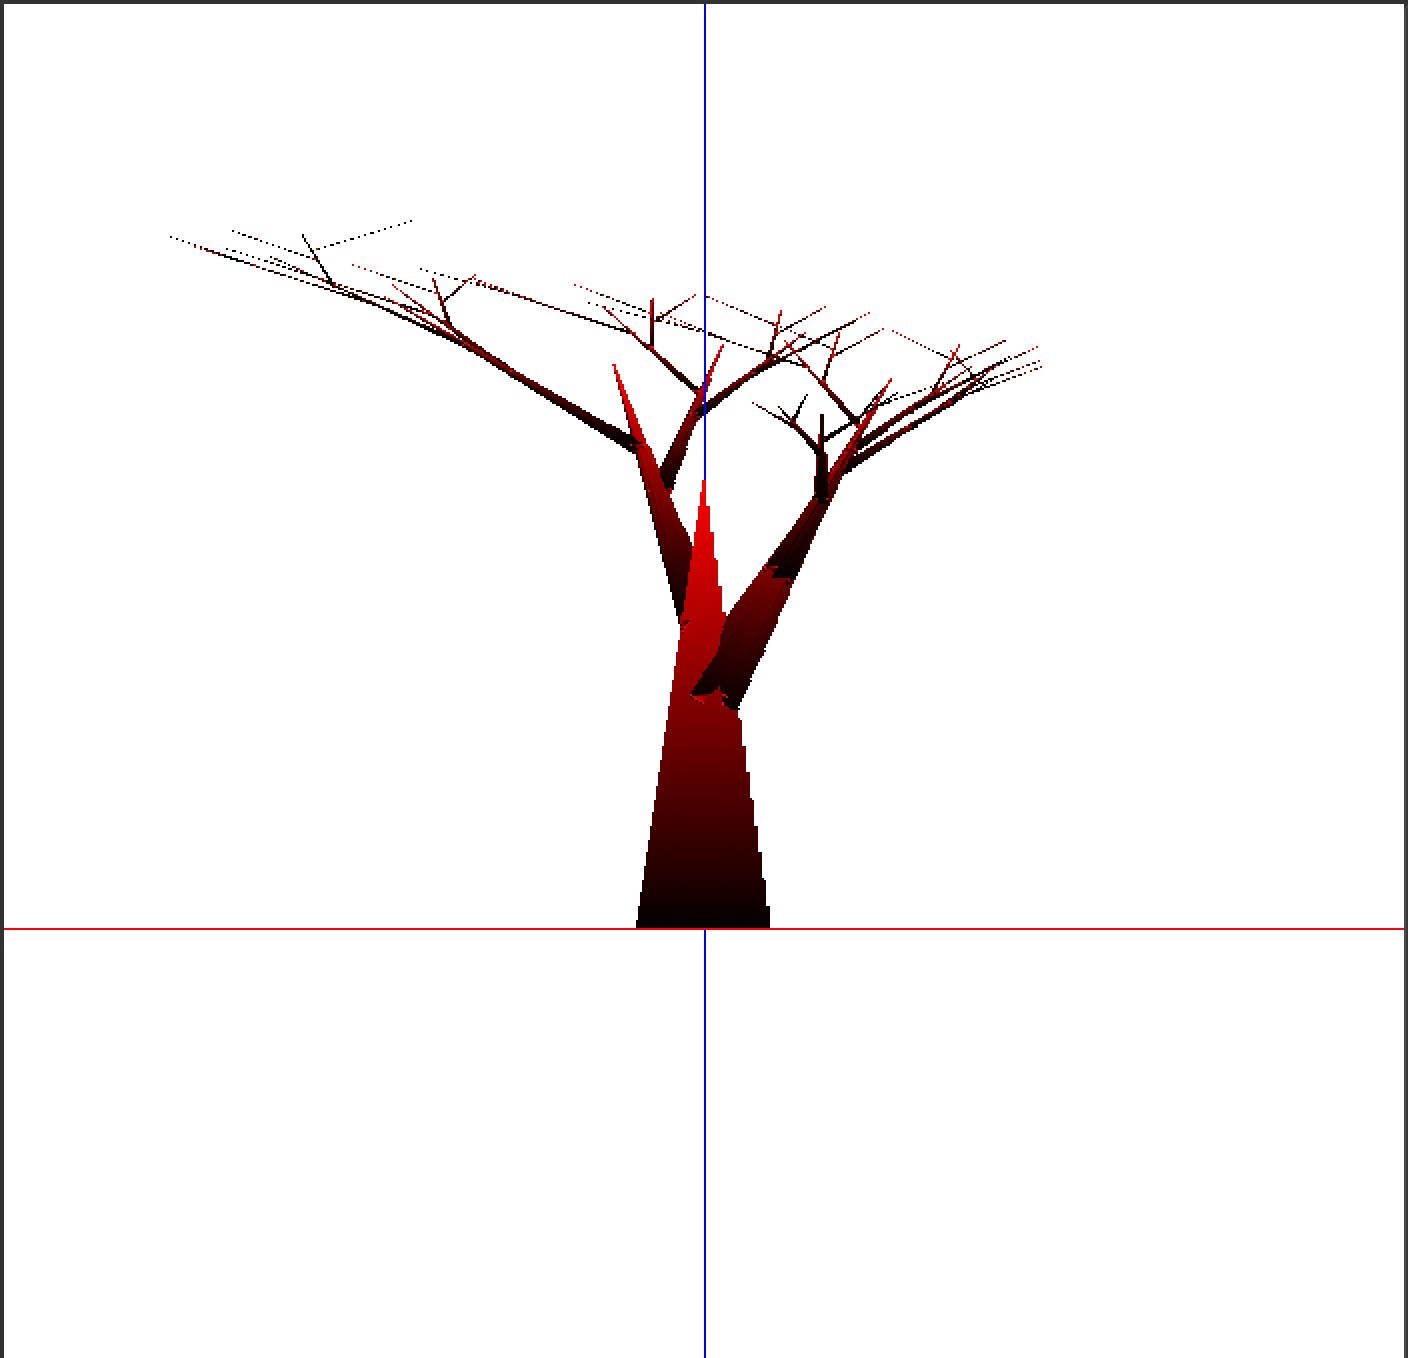
\includegraphics[scale=0.2]{img/ex1.JPG}
		\caption{Пример работы программы}
		\label{ris:ex1}
	\end{figure}

	\begin{figure}[ht!]
		\centering
		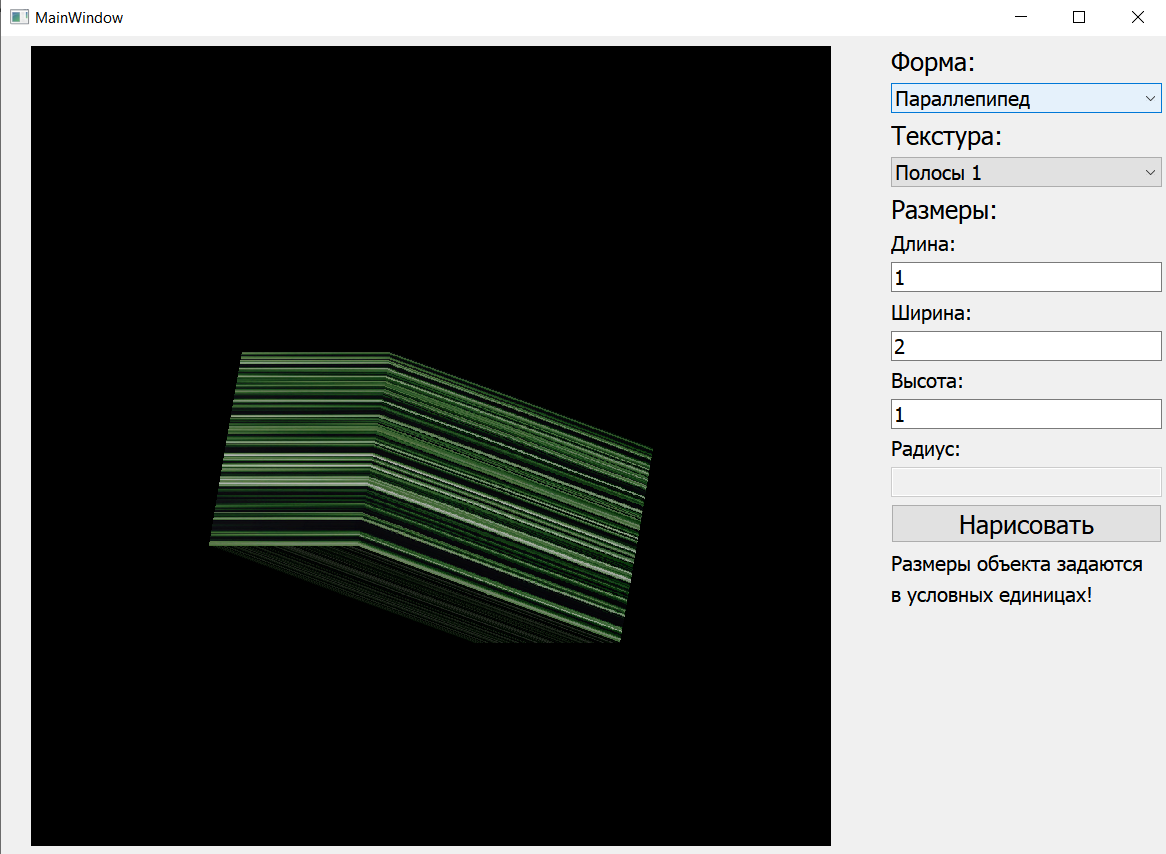
\includegraphics[scale=0.2]{img/ex2.JPG}
		\caption{Пример работы программы}
		\label{ris:ex2}
	\end{figure}

	\newpage

	\begin{figure}[ht!]
		\centering
		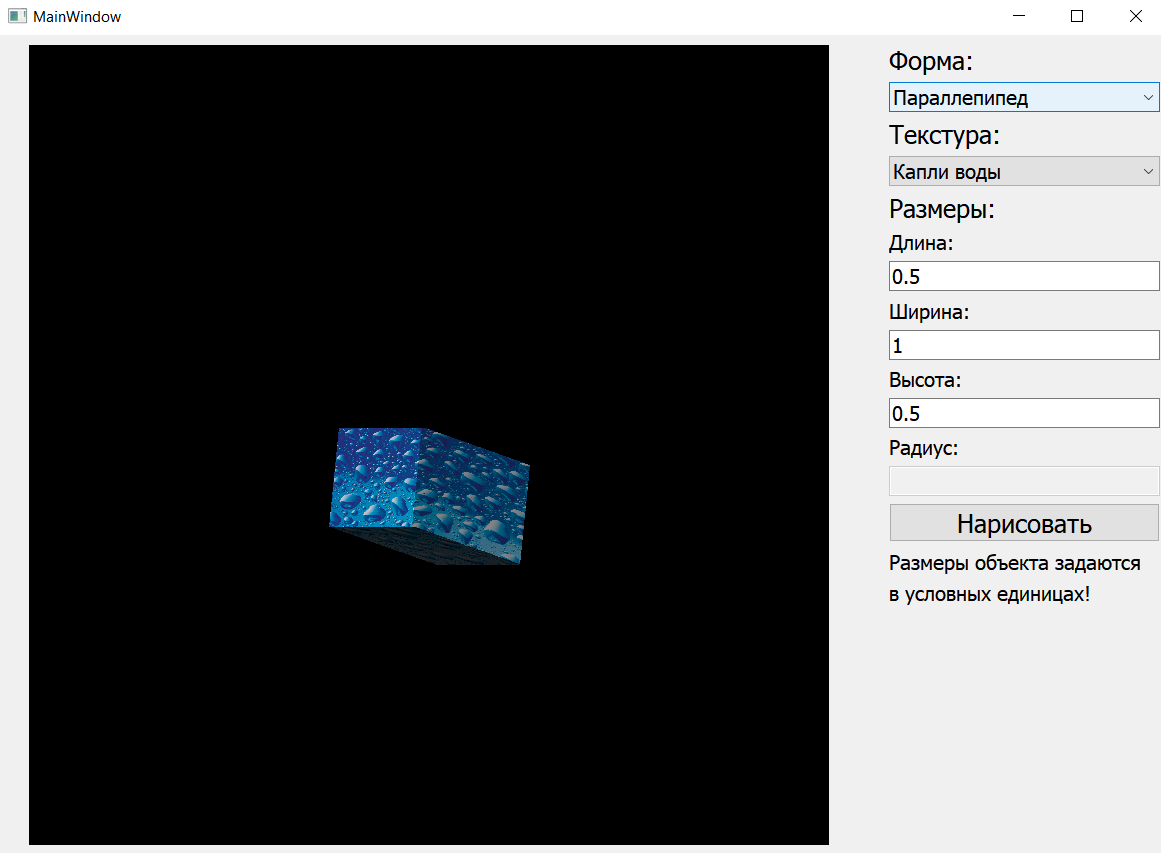
\includegraphics[scale=0.2]{img/ex3.JPG}
		\caption{Пример работы программы}
		\label{ris:ex3}
	\end{figure}

	\begin{figure}[ht!]
		\centering
		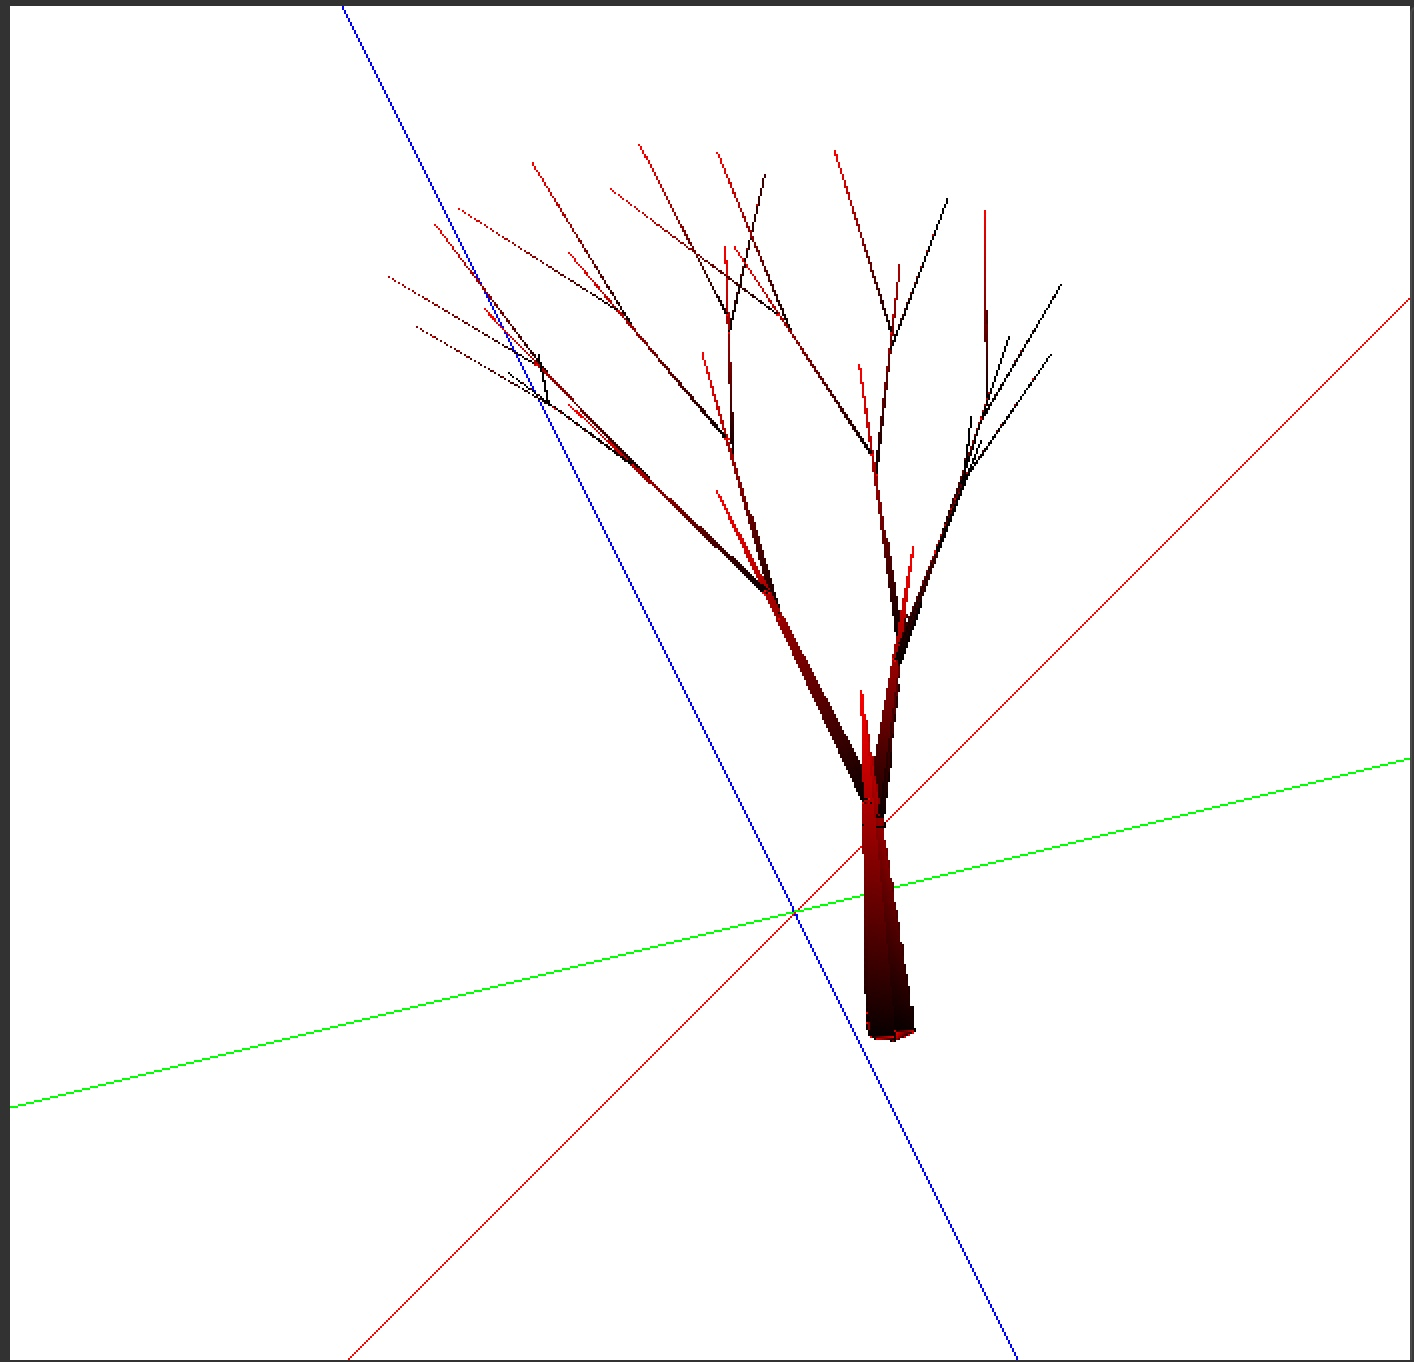
\includegraphics[scale=0.2]{img/ex4.JPG}
		\caption{Пример работы программы}
		\label{ris:ex4}
	\end{figure}

\newpage

	\begin{figure}[ht!]
		\centering
		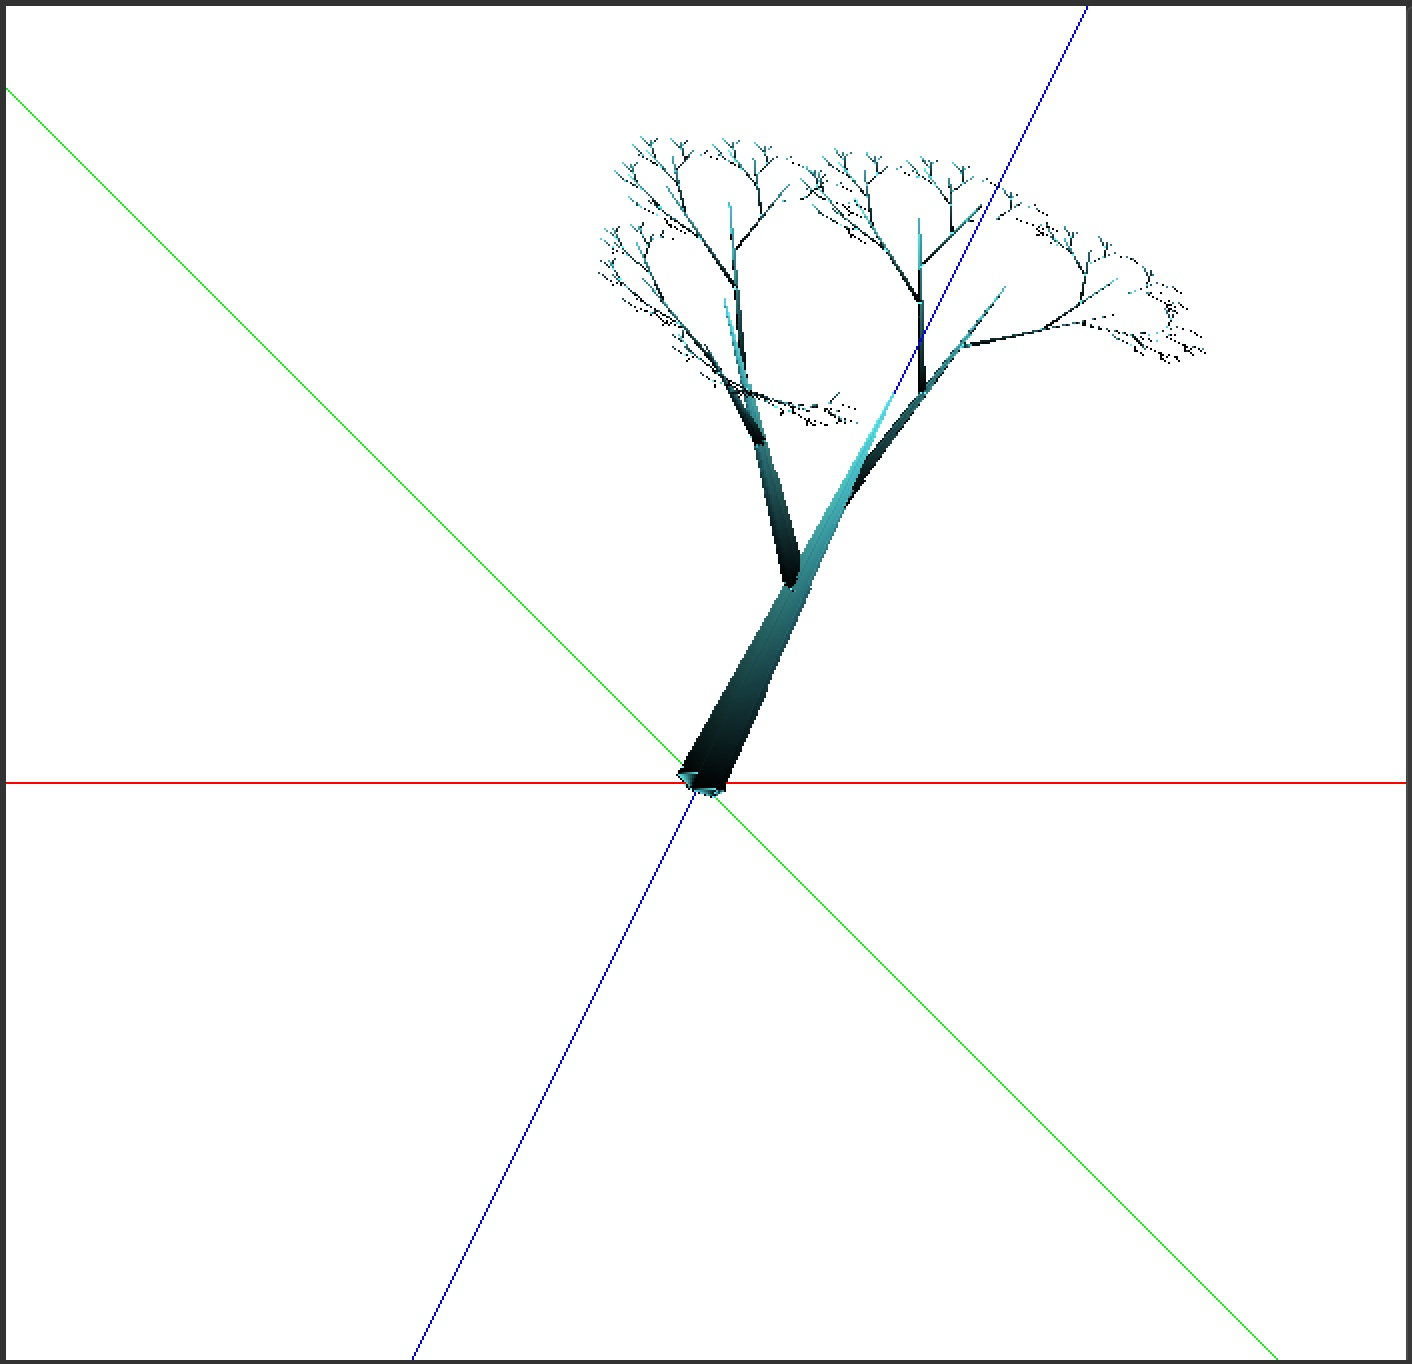
\includegraphics[scale=0.3]{img/ex5.JPG}
		\caption{Пример работы программы}
		\label{ris:ex5}
	\end{figure}

	\subsection{Выводы по технологическому разделу}
	В данном разделе были рассмотрены средства, использованные в процессе
	разработки для реализации поставленных задач, информация о сборке и запуске
	проекта, были представлены основные функции интерфейса, а также приведены
	примеры работы программы при различных параметрах.

	\newpage
	
	
	\section {Исследовательский раздел}
	В данном разделе будет проведено исследование временных затрат разработанного программного обеспечения в зависимости от количества потоков.
	\subsection{Исследование скорости работы алгоритма}
	Для исследования скоростных характеристик был использован компьютер на
	базе процессора Intel Core i7, с оперативной паматью 8 ГБ. Модуль
	тестирования запускался под операционной системой macOS Mojave.
	
	В таблице представлены данные, полученные в ходе замера времени работы алгоритма отображения одного и того же объекта при различном количестве граней конусов ствола и веток.
	
	\begin{table}[ht!]
		\begin{center}
			\begin{tabular}{ | c | c |}
				\hline
				Количество граней  & Время, тики \\ \hline  
				3 & 103259868\\   
				6 & 120575960\\      
				10 & 121135023\\    
				20 & 139548342\\
				50 & 203685764\\
				75 & 246526176\\
				100 & 315689052\\
				\hline
			\end{tabular}
		\end{center}
		\caption{Время работы алгоритма при разном количестве граней конусов ствола и веток}
	\end{table}

	\begin{tikzpicture}
	\begin{axis}[
	axis lines = left,
	xlabel = {Количество граней, шт},
	ylabel = {Время, тики},
	legend pos=north west,
	ymajorgrids=true
	]
	\addplot[color=blue, mark=square] table[x index=0, y index=1] {Time_work.dat};
	
	\addlegendentry{Время работы алгоритма}
	
	\end{axis}
	\end{tikzpicture}
	
	
	Очевидно, программа работает быстрее с меньшим количеством граней. Из данных графика можно сделать вывод, уже при 75 гранях программа работает почти 2.04 раз быстрее, чем при 6 гранях.
	
	\subsection{Выводы по исследовательскому разделу}
	В данном разделе было проведено исследование временных затрат разработанного программного обеспечения в зависимости от количества полигонов, на которые разбивается объект. Оно показало, что уже при разбиении конусов на 75 граней, алгоритм работает в 2 раза медленнее чем при 6 гранях.
	\newpage
	\section*{Заключение}
	\addcontentsline{toc}{section}{Заключение}
	В результате выполнения данного курсового проекта были изучены и реализованы генерация и моделирование деревьев. Была определена и описана предметная область работы, рассмотрены существующие методы и алгоритмы, из которых были
	выбраны подходящие для решения поставленной задачи, была сформирована архитектура проекта, спроектирован пользовательский интерфейс и реализовано требуемое ПО.
	
	В аналитическом разделе был произведён анализ предметной области, методов и алгоритмов, которые необходимы для решения поставленной задачи. В конструкторском разделе были подробно описаны эти алгоритмы, были даны формулы поворота относительно каждой из трех осей, перечислены основные типы и структуры данных, использующиеся в проекте, а также представлена диаграмма классов архитектуры проекта. В технологическом разделе были рассмотрены средства, использованные в процессе разработки для реализации поставленных задач, информация о сборке и запуске проекта, были представлены основные функции интерфейса, а также приведены примеры
	работы программы при различных параметрах.
	\addto\captionsrussian{\def\refname{Список используемой литературы}}
	\newpage
	
	\addcontentsline{toc}{section}{Список используемой литературы}
    \begin{thebibliography}{9}
    \bibitem{tree_book} The Algorithmic Beauty of Plants. - Режим доступа: http://algorithmicbotany.org/papers/\#abop, свободный - (Дата обращения: 01.10.2019)
    \bibitem{honda_explain} L-systems. Моделирование деревьев. [Электронный ресурс] - Режим доступа: https://habr.com/ru/post/83373/, свободный - (Дата обращения: 11.12.2019)
    \bibitem{algo_rotate} Поворот вокруг произвольной оси в пространстве - Режим доступа: http://scask.ru/a\_book\_mm3d.php?id=60,  свободный - (Дата обращения: 11.10.2019)
   	\bibitem{rod}Роджерс Д., «Алгоритмические основы машинной графики»/Роджерс Д.
   	- Москва: Издательство «Мир». Редакция литературы по математическим наукам,
   	1989
   	\bibitem{kur}Куров А.В. Курс лекций по машинной графике. – М., 201
    \bibitem{C} Докуменация C++ [Электронный ресурс]. - Режим доступа: https://cppreference.com/, свободный. (Дата обращения: 20.09.2019 г.)
    \bibitem{Qt} Документация QtCreator [Электронный ресурс]. - Режим доступа - https://doc.qt.io/, свободный. (Дата обращения: 20.09.2019 г.) 
	\bibitem{Guro} Основы освещения. [Электронный ресурс]. - Режим доступа: https://devburn.ru/2015/09/01/основы-освещения/, свободный  - (Дата обращения: 14.09.2019)    
	\bibitem{patterns} Паттерны проектирования [Электронный ресурс]. – Режим доступа: https://refactoring.guru/ru/design-patterns, свободный –
	(18.11.2019)
\end{thebibliography}
    
\end{document}